\documentclass[a4paper,11pt,final]{article}
% Pour une impression recto verso, utilisez plutôt ce documentclass :
%\documentclass[a4paper,11pt,twoside,final]{article}

\usepackage[english,francais]{babel}
\usepackage[utf8]{inputenc}
\usepackage[T1]{fontenc}
\usepackage[pdftex]{graphicx}
\usepackage{setspace}
\usepackage{hyperref}
\usepackage[french]{varioref}
\usepackage{geometry}
\usepackage{fancyhdr}
\usepackage{amsthm}
\usepackage[autostyle]{csquotes}
\usepackage{color}

\pagestyle{fancy}
\lhead{Thibaud COURTOISON}
\rhead{Rapport de stage de fin de DUT}

\geometry{hmargin=2.5cm,vmargin=2.5cm}

\newcommand{\reporttitle}{Rapport de Stage de fin de DUT}     % Titre
\newcommand{\reportauthor}{Thibaud \textsc{Courtoison}} % Auteur
\newcommand{\reportsubject}{Stage de fin d'étude} % Sujet
\newcommand{\HRule}{\rule{\linewidth}{0.5mm}}
\setlength{\parskip}{1ex} % Espace entre les paragraphes

%for quoting
\newenvironment{aquote}[1]{
  \pushQED{#1}
  \begin{quotation}
  }{
  \par\nointerlineskip\noindent\hfill(\popQED)
  \end{quotation}
}

%Nota Bene for me
\newcommand{\nb}[1]{\textcolor{red}{ #1 }}

\hypersetup{
    pdftitle={\reporttitle},%
    pdfauthor={\reportauthor},%
    pdfsubject={\reportsubject},%
    pdfkeywords={rapport} {vos} {mots} {clés}
}

\graphicspath{{../img/}}

\begin{document}
  % Inspiré de http://en.wikibooks.org/wiki/LaTeX/Title_Creation

\begin{titlepage}

\begin{center}

% Images entreprise & association
\begin{minipage}[t]{0.48\textwidth}
  \begin{flushleft}
    
\includegraphics [height=30mm]{logo-libertic.png} \\[0.2cm]
    \begin{spacing}{1.5}
      \textsc{\LARGE Association\\LiberTIC}
    \end{spacing}
  \end{flushleft}
\end{minipage}
\begin{minipage}[t]{0.48\textwidth}
  \begin{flushright}
    
\includegraphics [height=30mm]{logo-polypodes.png} \\[0.5cm]
    \textsc{\LARGE Entreprise\\Les Polypodes}
  \end{flushright}
\end{minipage} %\\[0.8cm]

\vfill

% Titre Rapport
\textsc{\Large \reportsubject}\\[0.5cm]
\HRule \\[0.6cm]
{\huge \bfseries \reporttitle}\\[0.4cm]
\HRule \\[1.0cm]

% Auteur et encadrant
\begin{minipage}[t]{0.3\textwidth}
  \begin{flushleft} \large
    \emph{Auteur :}\\
    \reportauthor
  \end{flushleft}
\end{minipage}
\begin{minipage}[t]{0.6\textwidth}
  \begin{flushright} \large
    \emph{Responsables :} \\
    M.~Ronan \textsc{Guilloux} \\
    M.~Nicolas \textsc{Hernandez}
  \end{flushright}
\end{minipage}


\vfill

\begin{minipage}[t]{0.48\textwidth}

  \begin{flushleft}
    
\includegraphics [height=30mm]{logo-univ.jpg} \\[0.2cm]
    \begin{spacing}{1.5}
      \textsc{\LARGE Université de Nantes}
    \end{spacing}
  \end{flushleft}

\end{minipage}
\begin{minipage}[t]{0.48\textwidth}

  \begin{flushright}
    
\includegraphics [height=30mm]{logo-iut.jpg} \\[0.2cm]
    \begin{spacing}{1.5}
      \textsc{\LARGE IUT de Nantes}
    \end{spacing}
  \end{flushright}

\end{minipage}
%\vfill

{\large Du 13 avril 2015 au 19 juin 2015}

\end{center}

\end{titlepage}

  \cleardoublepage % Dans le cas du recto verso, ajoute une page blanche si besoin
  \sloppy          % Justification moins stricte : des mots ne dépasseront pas des paragraphes
  \section*{Remerciements}
\addcontentsline{toc}{section}{Remerciements}

Je tiens tout d'abord à remercier les personnes qui m'ont accompagnés durant ces deux années de DUT.\\

\textit{M. Ronan Guilloux} et toute l'équipe des Polypodes, pour m'avoir accordé leurs confiance en m'acceptant dans leur équipe et pour m'avoir accompagné durant ces deux mois et demi. Leur patience et leur aide ont fait de ce stage une expérience particulièrement constructive.\\

Et bien sûr, toute l'équipe pédagogique du département informatique de l'IUT de Nantes, qui m'ont fait découvrir les mondes passionnants de l'informatique, de la gestion, du droit et de la communication. Si ces deux années peuvent s'assimiler à une réussite, c'est en très grande partie grâce à eux.\\

\nb{Refact this}

  \cleardoublepage
  \part*{Résumé du rapport}
\addcontentsline{toc}{section}{Resumé}

\section*{Résumé français}

Ce document est le rapport de mon expérience de deux mois et demi dans l'élaboration du projet Open Data Event en collaboration avec LiberTIC, une association nantaise militant dans l'Open Data, et Les Polypodes, une agence web promouvant le Logiciel Libre, située sur l'Île de Nantes. Vous trouverez dans un premier temps la présentation du stage et du projet. La suite vous présentera la phase d'Analyse et de Conception que j'ai effectuée. Puis, je décrirai la phase de Développement avec les différentes technologies que j'ai pu aborder. Enfin, une partie présentera les possibilités de suite du projet. Et pour finir, je ferai un bilan du projet, ainsi qu'un bilan personnel.

\section*{English abstract}

This document is a report of my two month and a half experience in the making of the Open Data Event project in collaboration with LiberTIC, a Nantes-based organization activist in the Open Data field, and Les Polypodes, a web agency promoting Free Software, located at L'Île de Nantes. First, you will find a presentation of the internship and the projet. The following will present the analysis and design phases I made. Then, I will describe the development stage with different technologies I had the possibility to tackle. Finally, a section will present the probable future of the project. And at the end, I will do a review of the project and a personnal assessment.
  \cleardoublepage
  \section*{Sommaire}
\addcontentsline{toc}{section}{Sommaire}

\tableofcontents 
  \cleardoublepage
  \section*{Introduction} % Pas de numérotation
\addcontentsline{toc}{section}{Introduction} % Ajout dans la table des matières

Ce document est un exemple de rapport écrit en \LaTeX.

Écrit par Thibaud Courtoison grâce à \url{http://blog.hikoweb.net/}.

Pour rajouter une correction ou une note, utiliser la commande \\ronan. Example:

\textbackslash{}ronan\{Tu as oublié de parler de XXX\}

va afficher:

\ronan{Tu as oublié de parler de XXX}
  \cleardoublepage
  \section{Le projet}

Une des particularités de mon stage est le fait que je travaillais en collaboration direct non seulement avec l'entreprise accompagnait mon stage, mais aussi avec des réprésentants de l'association LiberTIC, clients du projet. Cette section présentera donc Les Polypodes et LiberTIC, puis, je parlerais du projet, de ses premières versions et enfin de ma place sur ce projet.

\subsection{Données Ouvertes et LiberTIC}

\begin{aquote}{Wikipédia}
``L'ouverture des données (en anglais open data) représente à la fois un mouvement, une philosophie d'accès à l'information et une pratique de publication de données librement accessibles et exploitable.''
\end{aquote}

\subsection{Logiciel Libre et Les Polypodes}

\begin{aquote}{Wikipédia}
``Un logiciel libre est un logiciel dont l'utilisation, l'étude, la modification et la duplication en vue de sa diffusion sont permises, techniquement et légalement.''
\end{aquote}

\subsection{L'aggrégateur d'événement (ODE)}

\subsection{Les premières versions}

\subsection{Ma place sur le projet}
  \cleardoublepage
  \section{Analyse et Conception}

Comme tout projets de développement, il faut commencer par une phase d'analyse et de conception. Le projet Open Data Event a comme particularité d'avoir déjà eu plusieurs versions avant que je ne commence à travailler dessus. C'est pourquoi la partie d'analyse des versions précédentes était très importante, comme vous pourrez le lire par la suite.

\subsection{Mise en place de mon environnement de travail}

Il a été mis à ma disposition un \textbf{iMac} 21" avec un second écran de la même taille. J'ai donc pu découvrir l'environnement de développement offert par \textbf{OS X}. Globalement, la connaissance de l'environnement \textbf{Linux} m'aura aidé tout au long de l'utilisation d'OS X.

Après m'avoir créé un compte administrateur sur l'ordinateur fourni, j'ai pu installer tous les logiciels nécessaires à la réalisation du projet. Pour des raisons personnelles, j'ai choisi d'utiliser les outils suivants:

\begin{itemize}
    \item \textbf{iTerm} (Version 2.0.0)
    \item \textbf{Sublime Text 2} (Version 2.0.2)
    \item \textbf{Google Chrome} (Version 43)
    \item \textbf{Wireshark} (Version 1.12.5)
    \item \textbf{Apple Calendar} (Version 7.0)
    \item \textbf{PDFLatex} (Version 3.14)
\end{itemize}

Pour l'utilisation de serveurs SabreDAV, Baïkal, ElasticSearch et d'autres, j'ai installé une machine virtuelle avec \textbf{Vagrant}.

\textbf{LiberTIC} étant une association militant pour les licences libres, il était évident que la majorité de mon travail (qu'il s'agisse de développement ou de compte-rendus) soit mis lui aussi sous licence libre. Ainsi, il est possible de retrouver mon travail sur \textbf{GitHub} à l'adresse suivante: \url{https://github.com/LiberTIC/ODEV2}.

En plus de mon environnement local, j'ai pu accéder à un serveur de pré-production hébergé par OVH.

\subsection{Mise à niveau préliminaire}

Dès le début de mon stage, il a été défini que le projet allait se construire sur des technologies que je ne connaissais pas et/ou ne maitrisais pas. C'est pourquoi il a été convenu que la première semaine de mon stage serait consacrée à une mise à niveau pour différentes technologies.

Premièrement, j'ai suivi un récapitulatif des commandes \textbf{Git} \rf{gitimmersion} puis lu un article sur les bonnes pratiques de l'utilisation de Git et de ses branches \rf{successfulgit}.

Ensuite, j'ai lu plusieurs articles sur les bonnes pratiques du développement \textbf{PHP} \rf{bestpracticephp} \rf{stupidvssolid}.

Enfin, j'ai lu et appliqué la totalité du \textbf{Symfony Book} \rf{symfonybook}. Il s'agit du document de référence dans l'apprentissage du Framework. Ce document est mis à jour très régulièrement et permet d'obtenir une grande partie des informations nécessaires pour se lancer dans le développement d'une application Symfony 2.

\subsection{Analyse des besoins}

\subsubsection*{Service en ligne}

Une volonté de la part de LiberTIC était de faire d'ODE un service disponible en ligne. 
Sachant que j'ai effectué mon stage en partenariat chez Les Polypodes et que Symfony 2 est la Stack la mieux maitrisée par l'équipe, c'était le choix le plus logique pour pouvoir être accompagné par toute l'équipe en cas de besoins.

Symfony 2 est un framework PHP proposant un grand nombre de composants facilitant et accélérant le travail du développeur PHP.

\subsection{Conception et première réunion}

Une semaine après le début de mon stage, j'ai pu rencontrer deux personnes de l'association durant une réunion où nous avons discuté ensemble du périmètre du projet ainsi que ce que je proposais pour l'architecture.

\subsubsection*{CalDAV et WebDAV}

Dès la première réunion, il était clair qu'il fallait se baser sur un protocole déjà en place, pour ne pas `` réinventer la roue ''. Le seul protocole actuellement en place répondant à nos besoin est \textbf{CalDAV}. Il s'agit d'une extension du protocole WebDAV, lui même une extension du protocole HTTP (plus d'informations en Annexe 1). 

CalDAV définit la gestion des calendriers au sein d'un serveur. Il décrit aussi la façon dont les serveurs CalDAV doivent gérer les événements et les utilisateurs.

CalDAV est défini par la RFC 4791\rf{RFC4791} datant de 2007. Il existe plusieurs implémentations de cette RFC. La première, historiquement parlant, est CalendarServer, en python.

\subsubsection*{oEmbed}

Durant la réunion, nous avons discuté de la façon dont ODE devrait gérer l'ajout de médias à un événement. Après s'être mis d'accord sur le fait que gérer l'upload d'images, de vidéos ou autres, ne serait pas intéressant, M. Ségalou a évoqué l'utilisation d'oEmbed (\url{http://www.oembed.com/}).

oEmbed est un format permettant d'obtenir des informations relatives à un média. Globalement, il suffit de fournir une URL appartenant à un service compatible oEmbed (Youtube, Flickr, Vimeo, DailyMotion, SoundCloud, etc.) (Figure X). Ensuite, grâce à l'URL, il sera possible de récupérer des informations le concernant (Figure X). Pour enfin l'afficher directement sur le site (Figure X).

\newpage

\begin{figure}[H]
\begin{center}
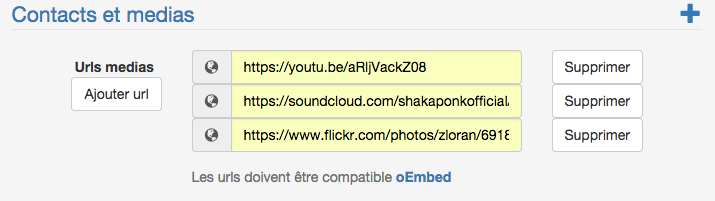
\includegraphics[height=30mm]{ajout_url_media.png}
\end{center}
\caption{Partie du formulaire pour ajouter des urls de médias}
\end{figure}


\begin{figure}[H]
\begin{lstlisting}[frame=single]
{
    "title": "Shaka Ponk - Wanna Get Free", 
    "width": 480, 
    "height": 270, 
    "thumbnail_height": 360, 
    "html": "\u003ciframe width=\"480\" height=\"270\" src=\"https:\/\/
www.youtube.com\/embed\/aRljVackZ08?feature=oembed\" frameborder=\"0\" 
allowfullscreen\u003e\u003c\/iframe\u003e", 
    "thumbnail_width": 480, 
    "author_url": "http:\/\/www.youtube.com\/user\/ShakaPonkVEVO", 
    "provider_name": "YouTube", 
    "version": "1.0", 
    "type": "video", 
    "provider_url": "http:\/\/www.youtube.com\/", 
    "author_name": "ShakaPonkVEVO", 
    "thumbnail_url": "https:\/\/i.ytimg.com\/vi\/aRljVackZ08\/
hqdefault.jpg"
}
\end{lstlisting}
\caption{Données récupérées depuis youtube grâce au format oEmbed}
\end{figure}

\begin{figure}[H]
\begin{center}
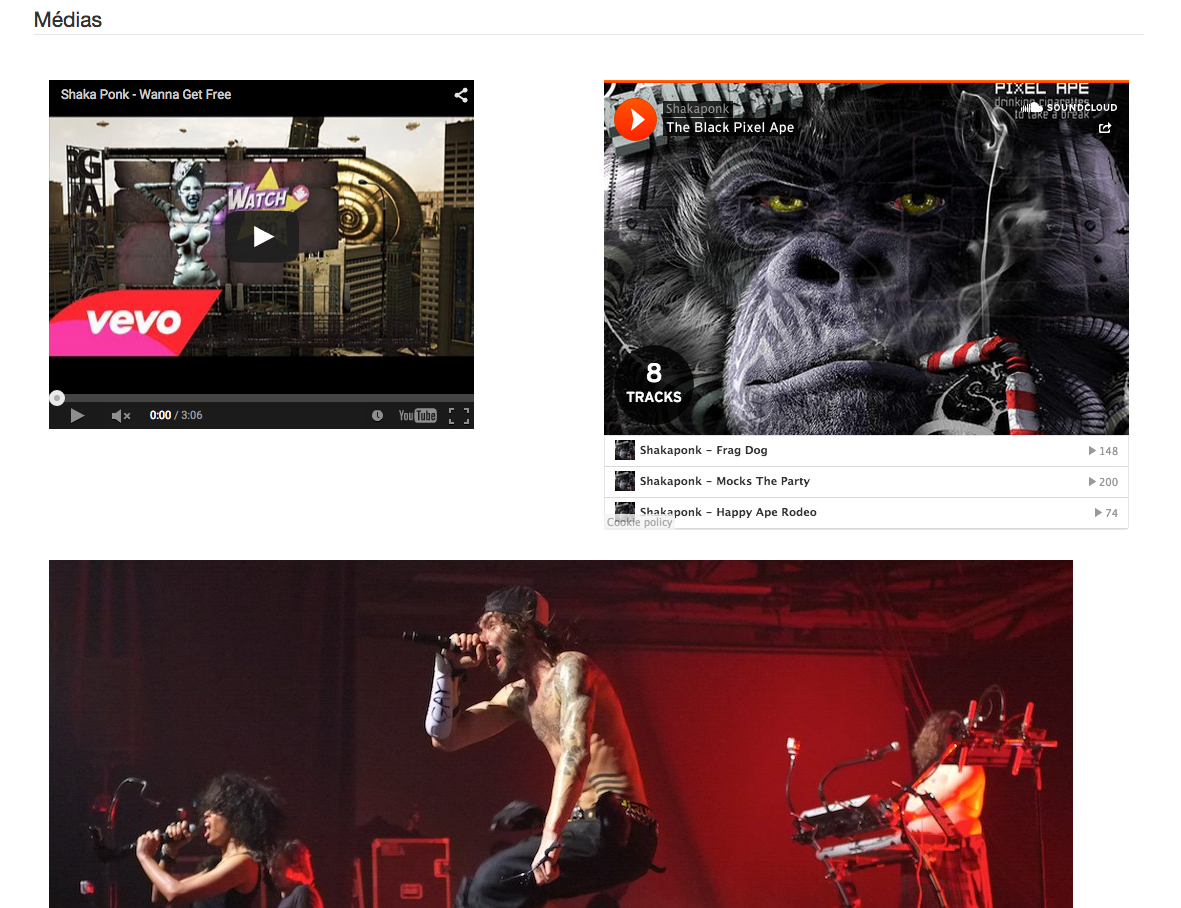
\includegraphics[height=70mm]{medias_embeded.png}
\end{center}
\caption{Médias affichés directement sur le site}
\end{figure}
  %\section{Analyse et conception}

Comme tous projets de développement, il faut commencer par une phase d'analyse et de conception. Le projet Open Data Event a comme particularité d'avoir déjà eu plusieurs versions avant que je ne commence à travailler dessus. C'est pourquoi la partie d'analyse des versions précédentes étais très importante.

\subsection{Environnement de travail}

J'ai effectué mon stage dans les bureaux de l'entreprise \textbf{Les Polypodes}, situés au 7\up{ème} de l'immeuble \textit{Sigma 2000}. Avec une vue panoramique sur l'île de Nantes, il fallait cependant ne pas se laisser divertir par les différents utilisateurs du terrain multi-sport en bas de l'immeuble.

Côté technique, il a été mis à ma disposition un \textbf{iMac} 21" avec un second écran de la même taille. J'ai donc pu découvrir l'environnement de développement offert par \textbf{OS X}. Globalement, la connaissance de l'environnement \textbf{Linux} m'aura aidé tout au long de l'utilisation d'OS X.

Après m'avoir créé un compte administrateur sur l'ordinateur fourni, j'ai pu installer tout les logiciels nécessaire à la réalisation du projet. Pour des raisons personnels, j'ai choisi d'utiliser les outils suivants:

\begin{itemize}
    \item \textbf{iTerm} (Version 2.0.0)
    \item \textbf{Sublime Text 2} (Version 2.0.2)
    \item \textbf{Google Chrome} (Version 43)
    \item \textbf{Wireshark} (Version 1.12.5)
\end{itemize}

Pour l'utilisation de serveurs SabreDAV, Baïkal, ElasticSearch ou autre (XXX citer la section correspondante XXX), j'ai installé une machine virtuelle grâce à \textbf{Vagrant}.

\textbf{LiberTIC} étant une association militant pour les licences libres, il était évident que la majorité de mon travail (qu'il s'agisse de développement ou de compte-rendus) soit mis lui aussi sous licence libre. Ainsi, il est possible de retrouver mon travail sur \textbf{GitHub} à l'adresse suivante: \url{https://github.com/LiberTIC/ODEV2}.

En plus de mon environnement local, j'ai pu accéder à un serveur de pré-production hébergé par OVH.

\subsection{Mise à niveau préliminaire}

Dès le début de mon stage, il a été défini que le projet allait se construire sur des technologies que je ne connaissais pas et/ou ne maitrisais pas. C'est pourquoi il a été convenu que la première semaine de mon stage devais me servir pour effectuer une mise à niveau pour différentes technologies.

Premièrement, j'ai suivi un récapitulatif des commandes \textbf{Git} \cite{gitimmersion} puis lu un article sur les bonnes pratiques de l'utilisation de Git et de ses branches \cite{successfulgit}.

Ensuite, j'ai lu plusieurs articles sur les bonnes pratiques du développement \textbf{PHP} \cite{bestpracticephp} \cite{stupidvssolid}.

Enfin, j'ai lu et appliqué la totalité du \textbf{Symfony Book} \cite{symfonybook}.

\subsection{Analyse des RFC}

Avant de commencer le projet, il fallait déjà que je comprenne toutes les technologies abordés. \textbf{CalDAV} étant la base du projet, j'ai du appronfondir mes connaissances sur le sujet.

Pour re-situer \textbf{CalDAV}, il s'agit d'une extension de WebDAV, elle-même extension du protocol HTTP. Globalement, elle défini et précise la façon d'envoyer des données au format \textbf{iCalendar} sur le réseau Internet.

\textbf{iCalendar}, quand à lui, est un format de fichier (.ical ; .ics ; .icalendar ). Il permet de stocker des événements (tels que "Cinéma à 16h" ou "Réunion service compta' tous les lundi à 9h"). Ce format est ensuite utilisé par des logiciels (tels que iCal, Google Calendar, etc..) pour en faire un affichage plus adapté aux utilisateurs.

Pour plus d'informations sur CalDAV et iCalendar, j'ai établi un "tutoriel" pour expliquer l'utilisation de chacun: \url{https://github.com/LiberTIC/ODEV2/blob/master/doc/Thibaud_Printemps2015/Tutoriel_Comprendre_CalDAV.md}

Pour effectuer ce travail d'analyse, j'ai du lire la presque-totalité des RFC suivantes:
\begin{itemize}
    \item \textbf{RFC 4918}: \url{https://tools.ietf.org/html/rfc4918}
    \item \textbf{RFC 4791}: \url{https://tools.ietf.org/html/rfc4791}
    \item \textbf{RFC 2324}: \url{https://tools.ietf.org/html/rfc2324}
\end{itemize}

\subsection{Analyse des versions précédentes}

Avant que je ne commence à travailler dessus, ce projet à traversé de nombreuses phases d'analyses, de conceptions et de développement.

\subsubsection*{La première réunion}

L'élément déclencheur de ce projet est la réunion du 11 juin 2014 à Stéréolux avec l'association LiberTIC et quelques acteurs de l'événementiel à Nantes. Il est apparu qu'il y avait une nécessité d'améliorer la diffusion des données.

C'est ainsi qu'est né le projet ODE (Open Data Event). Il s'agit d'un aggrégateur d'événement permettant de relier les fournisseurs d'événements (les organisateurs de festivals, concerts, conférence, etc...) avec les réutilisateurs d'événements (les utilisateurs de l'API, les journaux, etc...).

Cette réunion a permis de produire un cahier des charges pour le projet (disponible à cette addresse: \url{https://github.com/LiberTIC/ODEV2/blob/master/doc/Documents/120622_ODE_cahierDesCharges_MakinaCorpus.pdf} )

\subsubsection*{La première version}

Makina Corpus ( \url{http://makina-corpus.com/} ), entreprise de développement de logiciels libres, a répondu au cahier des charges en proposant de réaliser le projet. Plusieurs mois plus tard, la première version était fini et fut présenté à des responsable de l'association LiberTIC.

Cependant, durant la réunion, il est apparu de nombreuses différences dans la direction du projet mené par Makina Corpus avec la direction voulu par l'association. A la fin de la réunion, il a été décidé de ne pas continuer la relation entre l'association et l'entreprise.

\subsubsection*{La reprise par Les Polypodes}

Suite à une réunion de l'association LiberTIC abordant l'échec de la première version, Ronan Guilloux de l'entreprise Les Polypodes, présent à cette réunion, fit la proposition suivante: Les Polypodes serait prêt à accueillir des stagiaires pour effectuer le projet. Les stagiaires seraient accueilli par l'entreprise et l'association s'engagerait à faire un suivi plus approfondit du projet pour éviter la même fin que la version précédente.

\subsubsection*{Version 2 - Les premiers stagiaires}

En janvier 2015, deux stagiaires de BTS chez Les Polypodes ont commencé à travailler sur ODE version 2.

Leur travail a été de produire un prototype d'une application sous Symfony2 permettant une gestion des événements avec un serveur CalDAV. Ils ont fait un comparatif des serveurs CalDAV et fait une analyse des sémantiques disponibles pour les événements.

Sachant que la durée de leur stage n'était que de six semaines, ils n'ont pas pu faire évoluer le prototype ( disponible à cette adresse: \url{https://github.com/polypodes/CalDAVClientPrototype} )

\subsubsection*{Version 2 - Mon stage}

Depuis le 13 avril 2015, je travaille donc sur la version 2 du projet. Le but est de pouvoir réaliser le projet dans le temps qui m'est imparti ( 10 semaines ).

\subsection{Analyse cahier des charges}

Le 30 avril, j'ai participé à une réunion avec des représentants de l'association LiberTIC pour définir leurs besoins et leurs attentes quand à la réalisation de ce projet avec moi.

Durant cette réunion, je leur ai expliqué ce que j'avais effectué comme travail jusque là, je leur ai ensuite présenté plusieurs diagramme de conception UML, puis, nous avons discuté des points importants sur lesquels je devrai me focaliser durant mon stage.

\subsubsection{La partie serveur}

J'ai longtemps refléchi sur la pertinence d'utiliser CalDAV pour le projet. En effet, il s'agit d'une extension du protocol HTTP datant de plus de 15 ans qui n'est pas très utilisé.

Cependant, sachant que le partage des données doit être encouragé, il faut s'assurer que n'importe qui puisse inscrire des données dans ODE, que ce soit un(e) commercial(e), un(e) responsable technique ou un(e) secrétaire. Or, l'avantage de CalDAV est que de nombreux clients calendrier (dont Google Calendar et Apple Calendar) permet l'ajout d'un compte compatible CalDAV.

Ainsi, en utilisant CalDAV, nous pourrions disposer d'interfaces utilisateurs déjà optimisé pour la création et la gestion d'événements.

Le deuxième point que j'ai abordé durant la réunion du 30 avril fut la façon dont les événements serait stockés. J'ai d'abord pensé qu'une base de données SQL serait la façon la plus simple et efficace de stocker des événements. Cependant, en réfléchissant à la structure d'un événement (dont je parlerais plus tard), je me suis rendu compte que la structure ne convenait pas à un stockage linéaire comme SQL.

Après m'être renseigné sur les différentes alternatives à SQL, j'ai opté pour ElasticSearch (\url{https://www.elastic.co/}). Il s'agit d'un moteur d'indexation permettant un stockage au format JSON, idéal pour la structure d'un événement. De plus, grâce à ElasticSearch, il sera possible d'implémenter facilement une recherche d'événements par mot-clés.

\subsubsection{La partie application}

\subsection{Conception UML du projet}
  \cleardoublepage
  \section*{Conclusion}
\addcontentsline{toc}{section}{Conclusion}

Pour conclure, avec \LaTeX{} on obtient un rendu impeccable mais il faut s'investir pour le prendre en main.

  \cleardoublepage
  \phantomsection\addcontentsline{toc}{section}{Références}

\renewcommand{\refname}{Webographie}
\newcounter{firstbib}

\begin{thebibliography}{ABC}

    \bibitem{cartopendata} LiberTIC. \emph{OpenData Map}. URL: \url{http://www.opendata-map.org/}. Consulté le 1 juin 2015.

    \bibitem{gitimmersion} Gitimmersion. \emph{Best GIT tuto ever -50 steps}. URL: \url{http://gitimmersion.com/}. Consulté le 13 avril 2015.

    \bibitem{successfulgit} Vincent Driessen. \emph{A successful Git branching model}. Janvier 2010. URL: \url{http://nvie.com/posts/a-successful-git-branching-model/}. Consulté le 13 avril 2015.

    \bibitem{bestpracticephp} Brian Fenton. \emph{Best Practices for Modern PHP Development}. URL: \url{https://www.airpair.com/php/posts/best-practices-for-modern-php-development}. Consulté le 14 avril 2015.

    \bibitem{stupidvssolid} Hugo Hamon. \emph{Votre code est STUPID ? Rendez le SOLID}. Décembre 2013. URL: \url{http://afsy.fr/avent/2013/02-principes-stupid-solid-poo}. Consulté le 14 avril 2015.

    \bibitem{symfonybook} Sensio Labs. \emph{The Symfony Book}. URL: \url{http://symfony.com/doc/current/book/index.html}. Consulté plusieurs fois du 15 avril 2015 au 19 juin 2015.

    \bibitem{restsymfony} William Durand. \emph{REST APIs with Symfony2: The Right Way}. Août 2012. URL: \url{http://williamdurand.fr/2012/08/02/rest-apis-with-symfony2-the-right-way/}. Consulté le 22 mai 2015.

    \setcounter{firstbib}{\value{enumiv}}
\end{thebibliography}

\renewcommand{\refname}{RFCs}

\begin{thebibliography}{ABC}
    \setcounter{enumiv}{\value{firstbib}}

    \bibitem{rfc4918} RFC 4918. \emph{HTTP Extensions for Web Distributed Authoring and Versioning}. URL: \url{http://tools.ietf.org/html/rfc4918}.

    \bibitem{rfc4791} RFC 4791. \emph{Calendaring Extensions to WebDAV}. URL: \url{http://tools.ietf.org/html/rfc4791}.

    \bibitem{rfc6352} RFC 6352. \emph{vCard Extensions to WebDAV}. URL: \url{http://tools.ietf.org/html/rfc6352}.

    \bibitem{rfc5545} RFC 5545. \emph{Internet Calendaring and Scheduling Core Object Specification}. URL: \url{http://tools.ietf.org/html/rfc5545}

    \bibitem{rfc6350} RFC 6350. \emph{vCard Format Specification}. URL: \url{http://tools.ietf.org/html/rfc6350}.

\end{thebibliography}

  \cleardoublepage
  \section*{Annexes}
\phantomsection\addcontentsline{toc}{section}{Annexes}

\subsection*{Annexe 1 - Lexique}


\subsubsection*{Protocoles}

\underline{\textbf{WebDAV}} (ou \textbf{Web Distributed Authoring and Versioning}) est une extension du protocol \textbf{HTTP}. Il permet de récupérer, déposer, synchronier et publier des fichiers rapidement et facilement. WebDAV permet une édition de contenu simultanée avec plusieurs utilisateurs. WebDAV est décrit dans la RFC 4918\rf{RFC4918}.

\textit{Source: \blurl{http://en.wikipedia.org/wiki/WebDAV}{Wikipédia - WebDAV}}\\

\underline{\textbf{CalDAV}} (ou \textbf{Calendar Extensions to WebDAV}) est est un standard internet permettant à un client de planifier des informations sur un serveur distant. Il étend les spécifications de \textbf{WebDAV} et utilise le format \textbf{iCalendar} pour les données. CalDAV est décrit dans la RFC 4791\rf{RFC4791}.

\textit{Source: \blurl{http://en.wikipedia.org/wiki/CalDAV}{Wikipédia - CalDAV}}\\

\underline{\textbf{CardDAV}} (ou \textbf{vCard Extensions to WebDAV}) est un standard internet permettant à un client d'accéder et de partager des données de contacts sur un serveur disant. Il étend les spécifications de \textbf{WebDAV} et utilise le format \textbf{vCard} pour les données. CardDAV est décrit dans le RFC 6352\rf{RFC6352}.

\textit{Source: \blurl{http://en.wikipedia.org/wiki/CardDAV}{Wikipédia - CardDAV}}\\


\subsubsection*{Formats de fichiers}

\underline{\textbf{iCalendar}} est un format de fichier (.ical ; .ics ; .ifb ; .icalendar) permettant d'envoyer des événements entre utilisateur. iCalendar est indépendant du protocol de transport. En effet, le transport eut être effectué par mail, par partage sur un serveur \textbf{WebDAV} ou même par pigeon voyageur. iCalendar est décrit dans la RFC 5545\rf{RFC5545}.

\textit{Source: \blurl{http://en.wikipedia.org/wiki/ICalendar}{Wikipédia - iCalendar}}\\

\underline{\textbf{vCard}} est un format de fichier (.vcf ; .vcard) permettant de de transmettre des données personnelles (sous forme de Carte de visite). Le format vCal peut être utilisé en parallèle avec le format \textbf{iCalendar} pour lier des événements à des personnes. vCard est décrit dans la RFC 6350\rf{rfc6350}. La version actuelle est la 4.0, mais la 3.0 reste utilisé par de nombreux clients et serveurs.

\textit{Source: \blurl{http://en.wikipedia.org/wiki/VCard}{Wikipédia - vCard}}\\

\underline{\textbf{hCalendar}} (ou \textbf{HTML iCalendar}) est un microformat pour afficher une représentation HTML sémantique d'un calendrier au format iCalendar. L'avantage, outre un affichage personnalisé des événements, est la possibilité données à des outils de parsing d'extraire les informations pour les stocker sous le format souhaité (iCalendar ou autre). hCalendar est utilisé entre autres par Facebook, Google et Wikipédia.

\textit{Source: \blurl{http://en.wikipedia.org/wiki/HCalendar}{Wikipédia - hCalendar}}\\


\subsubsection*{Clients}

\underline{\textbf{iCal}} (renommé \textbf{Apple Calendar} depuis OSX Mountain Lion) est l'application de gestion de calendrier fait par Apple. Il peux entre autres, être client d'un serveur \textbf{WebDAV}.

\textit{Source: \blurl{http://en.wikipedia.org/wiki/Calendar_\%28application\%29}{Wikipédia - Calendar}}\\


\subsubsection*{Serveurs}

\underline{\textbf{SabreDAV}} est un serveur \textbf{CardDAV}, \textbf{CalDAV} et \textbf{WebDAV}. Il implémente les recommendations RFC actuelles. Il est compatible avec toutes les plateformes majeures.

\textit{Source: \blurl{http://en.wikipedia.org/wiki/SabreDAV}{Wikipédia - SabreDAV}}\\

\underline{\textbf{CalServ}}, aussi appelé \textbf{Calendars and Contacts Server} ou \textbf{Calendar Server} est un projet d'Apple d'implémentation des protocoles CalDAV et CardDAV. Sortie en 2006 sous le nom de iCal Server and Address Book Server, il a été porté sur des plateformes non-Apple. Il est écrit en Python et utilise une base de données SQL pour stocker les données.

\textit{Source: \blurl{http://en.wikipedia.org/wiki/Calendar_and_Contacts_Server}{Wikipédia - Calendar Server}}\\


\subsubsection*{Mix}

\underline{\textbf{Baïkal}} est une surcouche de SabreDAV. Il propose entre autres une interface d'administration web permettant la gestion du serveur CalDAV et CardDAV. Il est donc serveur et client de son propre serveur.

\textit{Source: \blurl{http://baikal-server.com/}{Site Baïkal}}

\clearpage

\subsection*{Annexe 2 - Modèle Evénement}


\begin{table}[h]
\begin{adjustwidth}{-1.8cm}{}
\begin{tabular}{|l || c | l | l | l |}

\hline
{\bf Propriété}&{\bf Type}&{\bf Description}&{\bf Source}&{\bf Exemple}\\
\hline
\hline

{\bf Base} &  &  &  &  \\

Nom & Texte & Nom court de l'événement & iCalendar & Concert Shakaponk \\
UID & Nombre & Identifiant Unique de l'event & iCalendar & SL-2015-XYZ-004 \\
Description & Texte & Description de l'événement & iCalendar & Concert de rock avec {[}...{]} \\

\hline

{\bf Date et heure} &  &  &  &  \\

Date début & Date & Date et heure de début & iCalendar & 2015-06-20 / 20:00 \\
Date fin & Date & Date et heure de fin & iCalendar & 2015-06-20 / 23:30 \\
Date création & Date & Date de création de l'event & ODE\_V2 & 2015-04-01 / 13:37 \\
Date modification & Date & Date de modif de l'événement & ODE\_V2 & 2015-04-03 / 20:15 \\

\hline

{\bf Localisation} &  &  &  &  \\

Lieu & Texte & Nom de l'endroit & iCalendar & Zénith Nantes \\
Emplacement & Texte & Nom de l'endroit & ODE\_V2 & Salle de concert \#3 \\
Géolocalisation & Geo & Géolocalisation de l'événement & iCalendar & 47.229234, -1.628550 \\
Capacité du lieu & Nombre & Capacité du lieu de l'event & ODE\_V1 & 4000 (personnes) \\

\hline

{\bf Organisation} &  &  &  &  \\

Participants & Texte & Participants à l'événement & schema.org & Shakaponk;Tagada Jones \\
Durée & Durée & Durée de l'événement & schema.org & PT3H30M (3h30min) \\
Status & Texte & Status de l'événement & iCalendar & Annulé / Reporté \\
Organisateur & Texte & Organisateur de l'événement & schema.org & Stéréolux \\
Sous-Evénement & UID & UID d'un sous-événement & schema.org & SL-2015-XYZ-009 \\
Super-Evénement & UID & UID d'un sur-événement & schema.org & SL-2015-XYZ-001 \\

\hline

{\bf URLs} &  &  &  &  \\

URL & URL & URL vers le site ODEV2 & iCalendar & http://ODEV2/event/XYZ004 \\
URL orga & URL & URL de l'event sur le site de l'orga & schema.org & http://stereolux/event/XYZ004 \\
URLs médias & URLs & URL de média compatible oEmbed & schema.org & http://website/image.jpg \\

\hline

{\bf International} &  &  &  &  \\

Langue & Texte & Langue de l'événement & ODE\_V1 & FR \\

\hline

{\bf Tarifs} &  &  &  &  \\

Prix standard & Nombre & Prix au tarif normal & ODE\_V2 & 10 \\
Prix réduit & Nombre & Prix au tarif réduit & ODE\_V2 & 7.5 \\
Prix enfant & Nombre & Prix au tarif enfant & ODE\_V2 & 5 \\

\hline

{\bf Contacts} & &  &  &  \\

Contact - Nom & Texte & Nom du contact & ODE\_V1 & John Smith \\
Contact - Email & Email & Email du contact & ODE\_V1 & john.smith@email.com \\

\hline

{\bf Catégorisation} & &  &  &  \\

Catégorie & Texte & Catégorie de l'événement & ODE\_V1 & Concert \\
Tags & Texte & Tags de l'événement & ODE\_V1 & Rock;Alternatif;{[}...{]} \\

\hline

\end{tabular}
\end{adjustwidth}
\end{table}

\end{document}